\documentclass{mystyle} % 使用自定义文档类
\usepackage{longtable}
\usepackage{array}
\usepackage{booktabs}
\usetikzlibrary{calc}


\renewcommand{\papertitle}{论文题目}
\renewcommand{\courseinfo}{课程名称(课程代码)}
\renewcommand{\semester}{2023-2024学年 第一学期}
\renewcommand{\studentname}{张三}
\renewcommand{\studentid}{12345678}
\renewcommand{\completiondate}{2024年12月20日}

\begin{document}
\maketitlepage

\begin{center}
\textbf{\fontsize{18}{22}\selectfont 这是标题}
\end{center}

% 内容提要部分
\begin{flushleft}
\fontsize{10.5}{12}\selectfont \textbf{内容提要:}请在这里写摘要
\end{flushleft}

% 关键词部分
\begin{flushleft}
\fontsize{10.5}{12}\selectfont \textbf{关键词:}请在这里写关键词
\end{flushleft}

% 正文部分
\setcounter{table}{0}
\section{第一个一级标题}
这里是正文部分,内容按照要求进行书写。正文的文字应为12号字,不加粗,行间距固定为20pt(图\ref{fig:1})。

\begin{figure}[htbp]
  \centering
  \begin{minipage}[t]{0.45\textwidth}
    \centering
    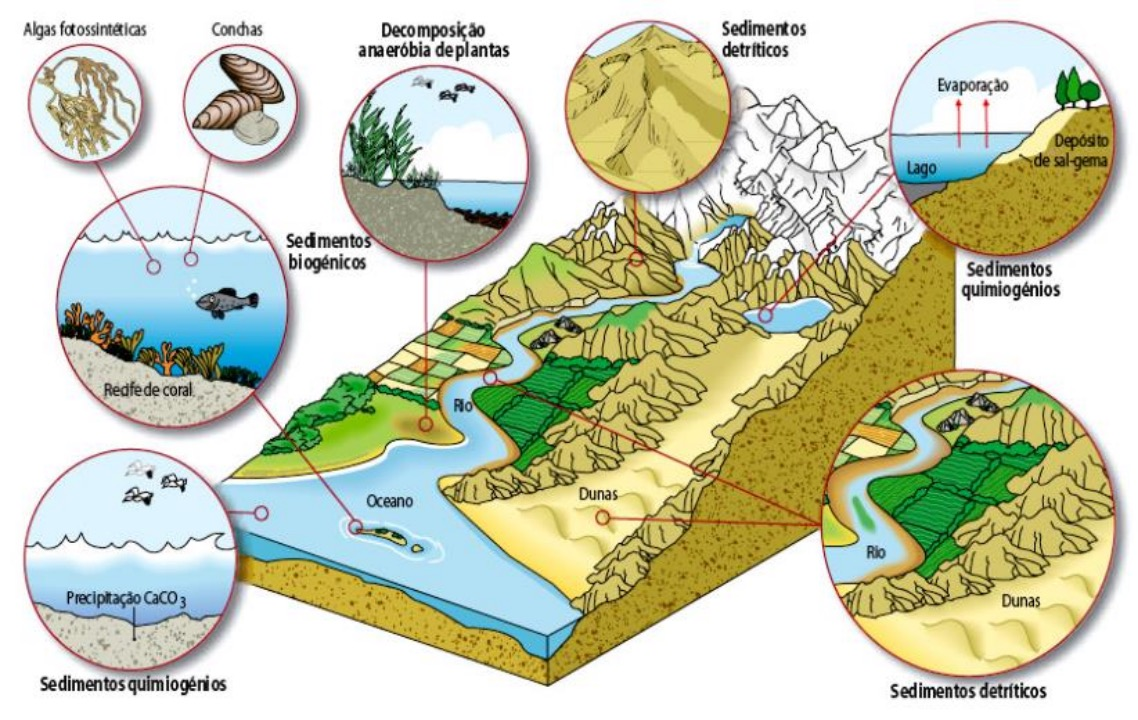
\includegraphics[width=\linewidth]{img/1.jpg}
\caption{需要引用的图片一,为了美观采用minipage插入}
\label{fig:1}
  \end{minipage}
  \hfill
  \begin{minipage}[t]{0.45\textwidth}
    \centering
    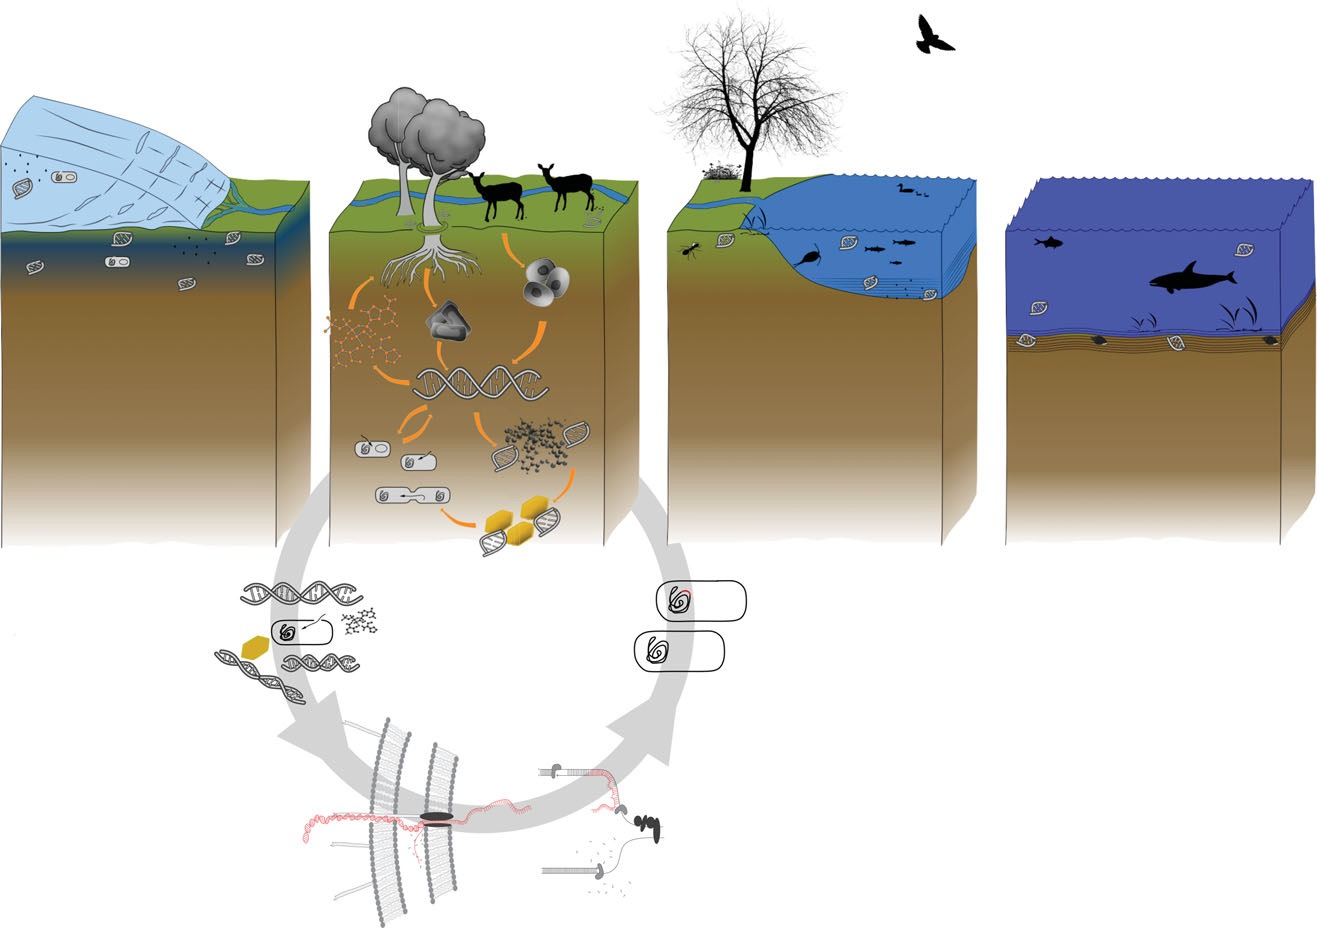
\includegraphics[width=\linewidth]{img/2.jpg}
\caption{需要引用的图片二}
\label{fig:2}
  \end{minipage}
\end{figure}
\subsection{二级标题}
\subsubsection{三级标题}
\section{第二个一级标题}
第二部分的正文内容,同样遵循上述格式要求。每个部分按照一级标题进行标注。以下是表格示例(表\ref{tab:grain size})。

\begin{table}[ht]
     \centering
     \caption{\label{tab:grain size}Sediment sample grain size analysis results}
     \begin{tabularx}{\textwidth}{lXXXXXX} % 使用 tabularx 和 X 列类型
     \hline
      \textbf{Sample} & \textbf{Md/μm} & \textbf{$\sigma$/μm} & \textbf{Clay (\%)} & \textbf{Silt (\%)} & \textbf{Sand (\%)} & \textbf{Gravel} \\
     \hline
     GS-sp1 & 154.204 & 207.387 & 5.21 & 21.04 & 73.75 & 0 \\
     GS-sp2 & 157.124 & 216.721 & 4.63 & 20.13 & 75.24 & 0 \\
     GS-sp3 & 134.061 & 160.691 & 5.09 & 25.74 & 69.17 & 0 \\
     General  & 148.463 & 194.933 & 4.98 & 22.30 & 72.72 & 0 \\
     \hline
     \end{tabularx}
\end{table}




\section{第三个一级标题}
继续写正文内容,确保每个段落之间无空行\cite{example1}。参考文献格式为国标。



\newpage
\printbibliography[heading=bibliography,title={参考文献}]

\end{document}
